 \documentclass[../ManualeSviluppatore_v1.0.0.tex]{subfiles}

\begin{document}

\section{Architettura}

	\subsection{Architettura generale}
		\subsubsection{Schema architettura generale}
			\begin{figure}[!h]
				\centering
				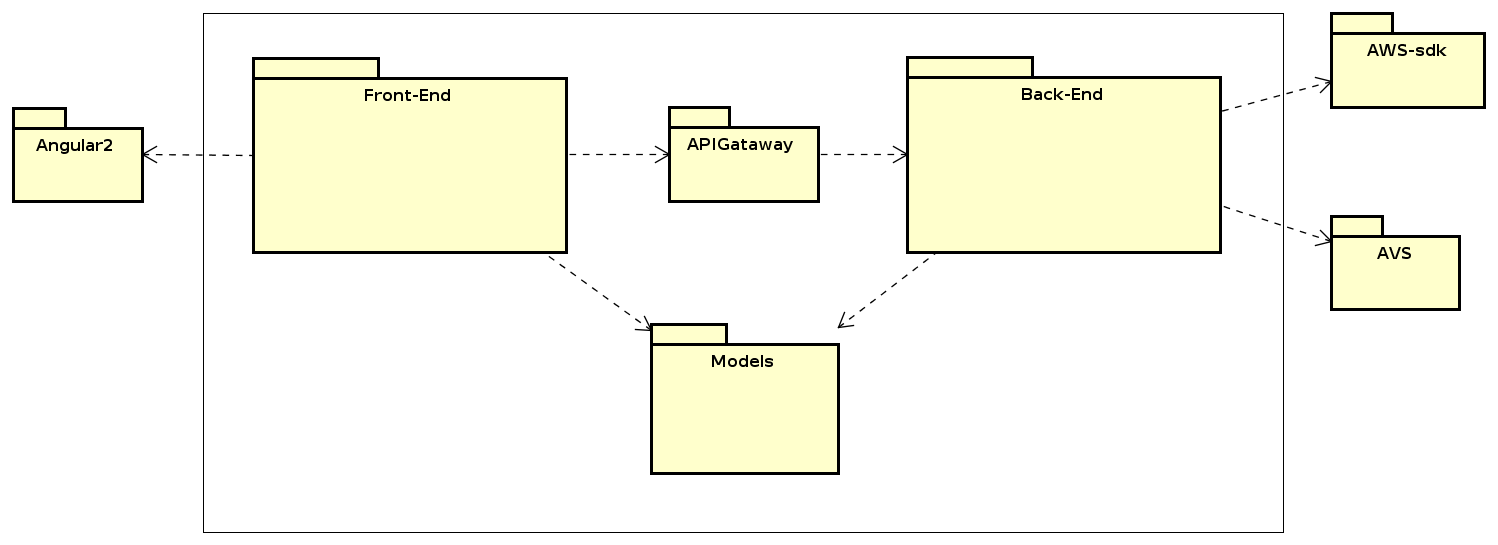
\includegraphics[width=\textwidth]{Architettura/AltoLivello.png}
				\caption{Schema architettura generale}
			\end{figure}

		\subsubsection{Descrizione}
		Nell'esposizione dell'architettura dell'applicazione si procederà con un approccio \gls{top-down}, descrivendola dal generico al particolare. Si inizia quindi dalla descrizione dei package e dei componenti, per poi descrivere nel dettaglio le singole classi, specificando per ognuna il tipo, l'obiettivo, la funzione.

		\subsubsection{Suddivisione logica}
			Durante la progettazione si è deciso di adattare diversi \gls{design pattern architetturali},
			difatti secondo le nostre esigenze, non era possibile adottarne uno univoco per l'intera architettura.
			Il sistema è quindi stato suddiviso in due parti:
			\begin{itemize}
				\item \textbf{Front-end}: la parte client del sistema, che deve essere eseguita da un qualsiasi browser, e verrà sviluppata con l'uso di AngularJS.
				\item \textbf{Back-end}: la parte risiedente nei sistemi cloud di Amazon, che eseguono l'elaborazione e forniscono i dati che verrà invece sviluppata in NodeJS e sfruttando i servizi distribuiti Amazon Web Service.
			\end{itemize}

		\subsubsection{Librerie e Framework}
			Di seguito verranno elencate le librerie ed i framework utilizzate per la realizzazione dell'intera Architettura.
			\begin{itemize}
				\item AngularJS
				\item Node.js
				\item AWS
				\item AVS
				\item RecordRTC
				\item AJV
				\item Alexa-app
				\item Fast Levenshtein
				\item Mocha
				\item Chai
				\item Chai-As-Promised
				\item Bootstrap
			\end{itemize}

\end{document}